%% This template can be used to write a paper for
%% Computer Physics Communications using LaTeX.
%% For authors who want to write a computer program description,
%% an example Program Summary is included that only has to be
%% completed and which will give the correct layout in the
%% preprint and the journal.
%% The `elsarticle' style is used and more information on this style
%% can be found at 
%% http://www.elsevier.com/wps/find/authorsview.authors/elsarticle.
%%
%%
%%\documentclass[preprint,12pt]{elsarticle}

%% Use the option review to obtain double line spacing
%% \documentclass[preprint,review,12pt]{elsarticle}

%% Use the options 1p,twocolumn; 3p; 3p,twocolumn; 5p; or 5p,twocolumn
%% for a journal layout:
%% \documentclass[final,1p,times]{elsarticle}
%% \documentclass[final,1p,times,twocolumn]{elsarticle}
%% \documentclass[final,3p,times]{elsarticle}
%% \documentclass[final,3p,times,twocolumn]{elsarticle}
%% \documentclass[final,5p,times]{elsarticle}
 \documentclass[final,5p,times,twocolumn]{elsarticle}


\usepackage{amsmath, amssymb,amsbsy,amsfonts}
\usepackage{color}



\usepackage{longtable}
\usepackage{listings}
\usepackage[caption=false]{subfig}

%% if you use PostScript figures in your article
%% use the graphics package for simple commands
%% \usepackage{graphics}
%% or use the graphicx package for more complicated commands
\usepackage{graphicx}
%% or use the epsfig package if you prefer to use the old commands
%% \usepackage{epsfig}


%% The lineno packages adds line numbers. Start line numbering with
%% \begin{linenumbers}, end it with \end{linenumbers}. Or switch it on
%% for the whole article with \linenumbers after \end{frontmatter}.
 \usepackage{lineno}

%% natbib.sty is loaded by default. However, natbib options can be
%% provided with \biboptions{...} command. Following options are
%% valid:

%%   round  -  round parentheses are used (default)
%%   square -  square brackets are used   [option]
%%   curly  -  curly braces are used      {option}
%%   angle  -  angle brackets are used    <option>
%%   semicolon  -  multiple citations separated by semi-colon
%%   colon  - same as semicolon, an earlier confusion
%%   comma  -  separated by comma
%%   numbers-  selects numerical citations
%%   super  -  numerical citations as superscripts
%%   sort   -  sorts multiple citations according to order in ref. list
%%   sort&compress   -  like sort, but also compresses numerical citations
%%   compress - compresses without sorting
%%
%% \biboptions{comma,round}

% \biboptions{}

%% This list environment is used for the references in the
%% Program Summary
%%
\newcounter{bla}
\newenvironment{refnummer}{%
\list{[\arabic{bla}]}%
{\usecounter{bla}%
 \setlength{\itemindent}{0pt}%
 \setlength{\topsep}{0pt}%
 \setlength{\itemsep}{0pt}%
 \setlength{\labelsep}{2pt}%
 \setlength{\listparindent}{0pt}%
 \settowidth{\labelwidth}{[9]}%
 \setlength{\leftmargin}{\labelwidth}%
 \addtolength{\leftmargin}{\labelsep}%
 \setlength{\rightmargin}{0pt}}}
 {\endlist}

\journal{Computer Physics Communications}

\newcommand{\consoleline}[2][0.5cm]
{\vspace{#1}
\textit{{#2}}
\vspace{#1}
}


\begin{document}

\begin{frontmatter}

%% Title, authors and addresses

%% use the tnoteref command within \title for footnotes;
%% use the tnotetext command for the associated footnote;
%% use the fnref command within \author or \address for footnotes;
%% use the fntext command for the associated footnote;
%% use the corref command within \author for corresponding author footnotes;
%% use the cortext command for the associated footnote;
%% use the ead command for the email address,
%% and the form \ead[url] for the home page:
%%
%% \title{Title\tnoteref{label1}}
%% \tnotetext[label1]{}
%% \author{Name\corref{cor1}\fnref{label2}}
%% \ead{email address}
%% \ead[url]{home page}
%% \fntext[label2]{}
%% \cortext[cor1]{}
%% \address{Address\fnref{label3}}
%% \fntext[label3]{}

\title{Marlics: A finite difference liquid crystal simulation package}

%% use optional labels to link authors explicitly to addresses:
%% \author[label1,label2]{<author name>}
%% \address[label1]{<address>}
%% \address[label2]{<address>}

\author[a]{R. F. de Souza \corref{R. F. de Souza/Rafael S. Zola}}
\author[a]{E. K. Omori}
\author[a,b]{R. S. Zola}

\cortext[author] {Corresponding author.\\\textit{E-mail address:} EuOuZola@somewhere.edu}
\address[a]{Departamento de Física, Universidade Estadual de Maringá, Avenida Colombo 5790,
87020 - 900 Maringá – PR, Brazil}
\address[b]{Universidade Tecnologica Federal do Paraná, Rua Marcilio Dias 635, 86812-460 Apucarana, Paraná,
Brazil}

\begin{abstract}
  In this paper we present Marlics to the world. Marlics is a software
  written in C++ to solve the Beris-Edwards equation of
  nematodynamics without flow for both achiral and chiral nematic liquid
  crystals. The system solved by Marlics consists in the dynamical evolution for the Q-tensor in the Landau-de Gennes formalism for different geometries, including confined slab cells and spherical, liquid crystal droplets.  The program takes as input a descriptive file giving the
  simulations parameters and initial conditions generating a series of
  different snapshots. The code is organized in class modules which
  can be modified by the user base to attend their further needs.
  \textcolor{red}{Review the abstract after the paper is finished}
\end{abstract}

\begin{keyword}
%% keywords here, in the form: keyword \sep keyword
Liquid crystals \sep Landau-de Gennes \sep finite differences.

\end{keyword}

\end{frontmatter}

%%
%% Start line numbering here if you want
%%
 \linenumbers

% Computer program descriptions should contain the following
% PROGRAM SUMMARY.

{\bf PROGRAM SUMMARY}
  %Delete as appropriate.

\begin{small}
\noindent
{\em Program Title: MarLicS}\\

{\em Licensing provisions: GNU General Public License v3.0 (GPL) }\\

{\em Programming language:C++}\\

{\em Supplementary material: Complete instructions about program usage can be found in the user-guide. }\\
  % Fill in if necessary, otherwise leave out.

{\em Nature of problem: Marlics was developed to simulate liquid crystal devices via solution of the Beris-Edwards system of differential equations without flow.}\\
% Describe the nature of the problem here. \\

{\em Solution method:  The system of equations is solved using finite differences in both time and space. The time integration is performed using an explicit integrator with or without variable time-step.}\\
% Describe the method solution here.

{\em External routines: The code needs the GSL (Gnu scientific library), an implementation of the CBLas library and an implementation of the OpenMp library(optional).}\\


{\em Running time: From minutes to hours depending on the problem size.}

{\em Computer: Single or multi-core processor with shared memory.}\\

{\em RAM: From hundreds of megabytes to gigabytes depending on the problem size.}\\


{\em Restrictions: The code is parallelized using OpenMp, consequently it can only be run in parallel with shared memory  processors.}\\

{\em Additional comments: The source code comes with a Mathematica
  notebook with can be used to aid the user to implement additional
  interactions, boundary conditions or other situations situation not
  covered by the current software.}

\end{small}


%% main text
\section{Introduction}
\label{Introduction}

Newly discovered and synthesized materials were responsible for a silent revolution that took place over the past decades in optics and photonics. Although the fundamental laws of optics have been well stabilised for more than a century, only with the application of new, smart and responsive materials that remarkable applications and devices thrived on our daily lives.  Such applications include display devices [], data storage and diffraction gratings [], image processing [], lasers [], optical tweezers [], spatial light modulators [] and son many others. LCs stand out among such materials since they are excellent to perform these functions, among which they can selectively reflect or transmit incoming light depending on its state. Moreover, LCs are responsible materials that can be controlled by  external stimuli, so their optical state can be easily tuned. In LC displays (LCDs), one of the most common application, it is used electric fields to control the LC optical state \cite{wu2006fundamentals}. Furthermore, LCs are often thought as scaled labs to study different scenarios and systems, which include topology [], knots [], pattern formation [], nature mimicking [], geometrical frustration [] and many others.

%There are several types o LCDs, where the major difference among them is the distribution of electrodes on the device, and the inclusion of protrusions at the boundaries of the confining surface \cite{chen2011liquid}.

In general, the design of new devices or any experimental setup involving soft condensed materials require a great amount of experimentation
and empirical knowledge. Performing every trial with a real apparatus
would require an unpractical number of prototypes to construct and
test. As an alternative, researchers can turn to modeling
software to aid them in the discovery process. Before prototyping a device or a complex experimental setup, or even to understand empirical data, they can be conveniently simulated in a package in many different forms, thus saving time and resources.

There exist some commercially available software for simulation of LC under different geometries, specially focusing on display devices, for instance LC3D~\cite{anderson2001lc3d} and LCD
master\cite{LCDMaster}. These software provide out of the box capabilities for simulation and visualization. However, they lack the
possibility of modifications and extension by the user. Open sources alternatives have appeared in the recent years to fill this gap, for example, Licra \cite{Licra} is one of such
attempt. The Licra software is written in C and support a few modes of
use, however, its implementation is very monolithic, and, if the user
wants to change a simulation parameter, or a mode of operation, he/she
has to code it directly to the source code and recompile the
executable. Recently, another open source liquid crystal simulation
software has been released \cite{Sussman2019}. The program named
openQmin, performs the minimization of the liquid crystal energy,
searching for its minimum energy state. The program works in many
situations and can be fine tuned by the user via a script or a
graphical interface.  It has many desirable capabilities, and performs
very well, but the program is focused on static problems. However, in several situations the dynamical process leading to a determined state is very important, for instance, during the annealing of defects, or during the operation of a certain LC device, where knowing the time dependence from swithing from one state to another is crucial.

In this paper we present \textit{marlics}, which is an open source code
designed to simulate the dynamics of liquid crystal order
parameters written in terms of the Q-tensor and obeying the Landau-de Gennes formalism in the presence of an external electric field for achiral and chiral nematics. The code is written in C++ using an independent
system of classes, which provide the building blocks for the most
common cases, and provide a framework where the user can develop their
specific applications. The mode of operation is defined by a script which is passed to the software and allows the used to set the different geometries (slab, sphere), boundary conditions, and initial conditions.

\section{Theoretical background}

LCs are anisotropic materials which have a certain degree of
long range ordering. Nematic LCs present orientational order, but no
positional order. Its state can be described by a combination of scalar and vectorial fields.  The preferred direction, for uniaxial nematics, can be represented by a vector $\vec{n}$, representing the average alignment of the anisometric molecules composing the material, and, due to the non-polar organization, $\vec{n}$ and
$-\vec{n}$ are equivalent. In some circumstances, if the material is biaxial, the
liquid crystal presents a second preferred direction, which it is also
described by a vector $\vec{l}$, called co-director. The degree in which the system is ordered in the direction of $\vec{n}$ is given by
the scalar order parameter $S$, whereas the order parameter $P$
measures the degree of orientation in the co-director direction. In this way, when $S=1$ the system is
perfectly oriented along $\vec{n}$, while $S=0$ represents an isotropic liquid (no preferred orientation). It is also possible to have $S <0$, in this case the molecules of the LC are oriented on average perpendicular to the director $\vec{n}$. 

In the general continuum theory for chiral nematics, the energy associated with variation of $\vec{n}$ in space is given by the Frank density of energy:
\begin{align} \label{eq:frank_energy}\nonumber
  f_f(\vec{n})&=\dfrac{1}{2} K_{11} (\nabla \cdot  \vec{n})^2 + \dfrac{1}{2} K_{22} (\vec{n} \cdot \nabla \times \vec{n}+q_0)^2\\
 & +\dfrac{1}{2} K_{33} \left| \vec{n} \times \nabla \times \vec{n} \right|^2 
  +\dfrac{1}{2} K_{24}  \nabla \cdot \left(\vec{n} \times \nabla \times  \vec{n} +\vec{n} \cdot \nabla \vec{n} \right),
\end{align}
with $\lbrace K_{11}, K_{22}, K_{33},K_{24} \rbrace$ being the elastic
constants of splay, twist, bend and saddle-splay, respectively and $q_0$ is the natural wavevector for a chiral nematic phase. The above expression is frequently used to interpret experimental results in terms of the elastic constants.  Nevertheless, it does not take into consideration neither variations in space or with temperature of the scalar order parameters. In the Landau-de Gennes formalism, however, the density of energy $f_s(S)$ associated with the scalar order parameter $S$ is given by:
\begin{equation}
\label{2}
  f_L(S)=\dfrac{1}{2} a \left(T-T^* \right) S^2- \dfrac{b}{3} S^3+\dfrac{1}{4} c S^4 +\dfrac{1}{2} L (\nabla S)^2,
\end{equation}
where $a,b,c$ and $L$ are thermodynamics constants, $T$ is the system's temperature and $T^*$ is the virtual nematic-isotropic phase transition temperature. Notice that the above equation describes variations of $S$ in space and with temperature. The scalar order parameters $\lbrace S, P \rbrace$ and the director and co-director $\lbrace \vec{n}, \vec{l} \rbrace$ can be combined in a unique order parameter $\mathbf{Q}$ , which is a second rank tensor whose
elements are given by:
\begin{equation}\label{eq:tensorial_parameter}
  Q_{ij}=\dfrac{S}{2}( 3 n_{i} n_{j}- 1) + \dfrac{P}{2}(l_i l_j - m_i m_j),
\end{equation}
where $i=1,2,3$ and $j=1,2,3$ and $vec{m}$ is the third biaxial director.  This order parameter is symmetric and traceless, therefore only 5 independent elements, for example $\lbrace Q_{11}, Q_{12},Q_{13}, Q_{22}, Q_{23} \rbrace $, are necessary to fully determine it. Since the tensor $\mathbf{Q}$ contains all the elements of symmetry of a nematic phase, we may rewrite eq.~\eqref{2} in terms of the scalars formed by the trace of Q and its gradients. Therefore, deviations from the equilibrium value of the scalar order parameter, or
spatial variations of the director has an associate energy density,
given by Landau-de Gennes energy density, ($f_{LDG}(\mathbf{Q})$) as:
\begin{align}\label{eq:Landau_deGennes} \nonumber
  f_{LDG}(\mathbf{Q})&=\dfrac{a}{2}(T-T^*) \text{Tr}(\mathbf{Q}^2) +
                       \dfrac{B}{3} \text{Tr}(\mathbf{Q}^3)
                       +  \dfrac{C}{4} \text{Tr}(\mathbf{Q}^2)^2 \\ \nonumber
                     &+ \dfrac{1}{2} L_1 \left( \partial_i Q_{jk} \right)
                       \left( \partial_i Q_{jk} \right) + \dfrac{1}{2} L_2
                       \left( \partial_i Q_{ji} \right) \left( \partial_k Q_{jk} \right) \\
                     &+\dfrac{1}{2} L_3 Q_{ij}\left( \partial_i Q_{kl}\right) \left(\partial_j Q_{kl}\right)
                     +\dfrac{1}{2} L_s \left( \partial_k Q_{ij} \right)\left( \partial_j Q_{ik} \right)\\
                     &+ \dfrac{4 \pi}{P_0} L_q \epsilon_{ijk} Q_{ij}\left( \partial_j Q_{ik} \right)                     
\end{align}
where $Q_{ij,k}=\partial Q_{ij}/\partial x_k$, $\epsilon_{ijk}$ is
the Levi-Civita tensor, $\lbrace L_1 ,L_2,L_3, L_q, L_s \rbrace$ are
elastic constants (in the sense that they represent spatial variations of $\vec{n}$), $\lbrace a,B,C \rbrace$ are thermodynamic
constants related to the nematic isotropic transition and $P_0=2\pi/q_0$ is the natural pitch of the chiral nematic phase ($q_0=0$ if the material is achiral), thus the term with $L_q$ represents the chiral contribution to the free energy. Here we have used Einstein's summation convention on repeated indexes.

The elastic constants of the Frank energy $\lbrace K_{11}, K_{22}, K_{33}, K_{24} \rbrace$ and the Landau-De Gennes ones $\lbrace L_1 ,L_2,L_3, L_q, L_s \rbrace$ are related by the expressions [CITAR]:
\begin{align}\label{eq:frank_to_ldg} \nonumber
L_1&=\dfrac{2 (K_{33}-K_{11}+3 K_{22})}{(27 {S_{eq}}^2)}\\\nonumber
L_2&=\dfrac{4 (K_{11}-K_{22}-K_{24})}{(9 {S_{eq}}^2)}\\\nonumber
L_3&=\dfrac{4 (K_{33}-K_{11})}{(27 {S_{eq}}^3 )}\\\nonumber
L_q&=\dfrac{2 (K_{22})}{(9 {S_{eq}}^2)}\\
L_s&=\dfrac{4 (K_{24})}{(9 {S_{eq}}^2)}
\end{align}

The dielectric energy density is given by:
\begin{equation}
 f_e(\mathbf{Q})= -\dfrac{1}{3} \epsilon_0 \Delta \epsilon^m E_i E_j Q_{ij}+ \dfrac{\epsilon_0}{2}  \mathbf{E} \cdot \mathbf{E},
\end{equation}
where $\epsilon_0$ is the vacuum dieletric constant,
$\Delta \epsilon=\epsilon_{\parallel} - \epsilon_{\perp}$ is the
dielectric anisotropy, which measures the difference between the
dielectric constant parallel($\epsilon_{\parallel}$) and perpendicular
($\epsilon_{\perp}$) to the liquid crystal director.  The volume energy
density ($f_v$) will be given by the sum of all energy terms being considered:
\begin{equation}\label{eq:total_energy}
  f_v(\mathbf{Q})=f_{LDG}(\mathbf{Q})+f_e(\mathbf{Q})
\end{equation}

The liquid crystal also interacts with the confining surfaces, which
can induce an order parameter at the surface and a preferred direction
for the director, which is called surface easy axis $n_0$. One of the
simplest form of the surface energy density between a liquid crystal
and a surface is given by the Rapini-Papoular (also called Nobili-Durant) which is given by:
\begin{equation}
\label{RP}
  f_{RP}(\mathbf(Q))=\dfrac{1}{2} W_1 (Q_{ij}-Q^0_{ij}) (Q_{ij}-Q^0_{ij})
\end{equation}
where $Q_{ij}^0$ is the surface induced order parameter, which can be
given in its tensorial form, or constructed using the induced scalar
order parameters $\lbrace S^0, P^0 \rbrace$ and the induced easy axis
$\lbrace \vec{n}, \vec{l} \rbrace$ using expression
\ref{eq:tensorial_parameter}.

When the liquid crystals boundary is a liquid or gas, instead of
inducing a preferred direction, the surface may induce a preferred
plane of orientation perpendicular to the surface. Any variation of
the director inside this plane gives the same energy. This type of
surface energy is described by the Fournier-Galatola anchoring energy
given by \cite{Sec2012}:
\begin{equation} \label{eq:penalizacao}
f_{FG}(\mathbf{Q})=W\left( \tilde{Q_{ij}}(\mathbf{Q}) - \tilde{Q}_{ij}^{\perp}(\mathbf{Q}) \right)\left( \tilde{Q_{ij}}(\mathbf{Q}) - \tilde{Q}_{ij}^{\perp}(\mathbf{}{Q}) \right)
\end{equation}
where $W$ is the anchoring strength constant,
$\tilde{Q_{ij}}(\bold{Q})=Q_{ij}+\dfrac{S_0}{3} \delta_{ij}$ and
$\tilde{Q_{ij}}^{\perp}(\bold{Q})=(\delta_{ik}-\nu_i \nu_k)Q_{kl}
(\delta_{lj}-\nu_l \nu_j)$. Here $\vec{\nu}=\lbrace\nu_1,\nu_2,\nu_2 \rbrace$ is the normal surface vector.

The time evolution of the order parameter is given by the
Beris-Edwards set of equations. If we neglect the liquid crystal flow,
the time evolution of $Q_{ij}$ in the bulk will be given by:
\begin{equation} \label{eq:dissipacao_Q}
\dfrac{\partial Q_{ij}}{ \partial t} = -\dfrac{\Lambda_{ijkl}}{\mu} \left( \dfrac{\partial f_{V}(\mathbf{Q})}{\partial Q_{kl}} - \dfrac{\partial}{\partial x_m } \dfrac{\partial f_V(\mathbf{Q})}{\partial Q_{kl,m}}  \right)=F_{ij}(\mathbf{Q}),
\end{equation}
%
where $\mu$ is the bulk viscosity (related to the rotational viscosity), and $ \Lambda_{ijkl} = (\delta_{ik} \delta_{jl}+\delta_{jk} \delta_{kl}-2 \delta_{ij} \delta_{kl}/3)$. Meanwhile the dynamics in the bulk will be given by
\begin{align}\label{eq:dissipacao_Q_superficie}
\dfrac{\partial Q_{ij}}{\partial t}=-\dfrac{\Lambda_{ijkl}}{\mu_s}\left(\nu_m\dfrac{\partial f_{V}(\mathbf{Q})}{\partial Q_{kl,m}} -\dfrac{\partial f_{suf}(\mathbf{Q})}{\partial Q_{kl}}\right)=F^s_{ij}(\mathbf{Q}),
\end{align}
here $\mu_s$ is the surface viscosity, $\nu_m$ is the $m_{th}$ component of the normal to the surface, and $f_{suf}$ is the surface energy, which may be chosen to be eq.~\eqref{RP} or eq.~\eqref{eq:penalizacao}.

We solve solve the system of equations using the method of lines
\cite{Bhattacharjee2008}. In this method, the spatial and time
discretization of the governing equations are performed separately and
independently, and the spatial dimensions of the equations
discretized first.  We discretize the right-hand side of
\eqref{eq:dissipacao_Q} and
\eqref{eq:dissipacao_Q_superficie} by means of finite differences. In the bulk, we have taken centered differences for both first order and second
order derivatives. On the surface, we have taken centered differences
for derivatives perpendicular to the normal and first order to
derivatives parallel to the surface normal.

In the method of lines, the temporal discretization depends on the
kind of integrator intended to propagate the solution. In the current
version of Marlics, we have implemented only a explicit integrator,
thus we have approximated the time derivatives by forward differences.
As an example, we shall take the Euler method: By assuming $Q^t_{ij}$ is
the value $Q_{ij}$ at time $t$, the value of $Q^{t+\Delta t}_{ij}$ can
be calculated by:
\begin{align}
  Q^{t+\Delta t}_{ij}=Q^{t}_{ij}+ \Delta t F_{ij}(\mathbf{Q})
\end{align}

Although the Euler method is convergent and can be used in some cases,
it has its drawbacks. The value of $\Delta t $ is fixed during the
simulation, and the allowed timestep size is to small for some
applications. As an alternative we have provided another (SAO 3 INTEGRADORES?) 2 explicit
integrator with the program: xplicit second order Runge-Kutta, which
also has a fixed timestep but is more stable, and the Dormand-Prince
5(4), which has a self-adaptive timestep. We implemented the time
adaption as proposed in reference \cite{hairer2008solving}.

\section{Software Usage:} \label{sec:software_usage}

Here we present the basic information necessary to install and use the
software. The complete information about software usage can be found
in the supplementary material ``Userguide''.

\subsection{Installation:}

The installation of Marlics in Unix systems is very
straightforward. The source code comes with a \textit{makefile} to
help users compile it on the computer. Actually, the {\it makefile} provides
 automatic installation for two compilers (one of them is free).
The user will  just need to assure that the \textit{make}
software and the necessary external libraries and their respective
developer files are installed. These libraries are: GSL (Gnu Scientific
library), OpenMp (optional, but highly recommended) and a CBLAS
implementation (you can use the GSL implementation for example). If
everything is present, the user just need to open a terminal in the
program folder and type:
{\it
\begin{lstlisting}
  make
\end{lstlisting}
}
\noindent to compile the program. Once the compilation is done, the user will
find an executable named \textit{marlics} in the installation
folder. For ease of use, this executable can be added to one of the
system search paths for binaries files, or the user can add the
installation folder to the list of searchable paths. Its is also
possible to run the simulations in the same path that the software is installed, but this is not recommended.

\subsection{Simulation set up and Execution:}

To execute marlics, the user must call the program passing an input file, which sets the simulation parameter as follows:
\begin{lstlisting}
marlics intput_file
\end{lstlisting}
where \textit{input\_file} is the file containing the simulation
parameters.

We here provide an input files that the user can use to test the program, or as a base to their own simulations. All
the parameters necessary to set up the simulation must be passed to
the program via input file. An entry in the input file is set by passing the parameter's name
followed by the parameter's required values:
\begin{lstlisting}
parameter value
\end{lstlisting}
Comments may be placed in the input file by starting a line with ``\#'',
everything in this line will be ignored by marlics. Also, everything
following the required parameters will also be ignored by marlics. We
find it very useful to keep the parameters units after their values. Some parameters must be set, while others can have standard values associated with them. Whenever marlics use an standard value, it informs the user in the standard output what value has been used.
The standard values of the parameters and their units can be found in the table given in \ref{apx:list_of_parameters}. The simulation constants must be filled with a real number. The user has two options to pass the elastic constants: the user can pass the $L_i$ values (elastic constants in the Landau-de Gennes formalism), which are the constants actually used in the calculations, or to pass the $K_{ii}$ values (elastic constants in the Frank formalism) and let marlics calculate $L_i$. 
Also, the chirality power can be passed in two different ways, as $p_0$, i.e the pitch, or as $q_0$, i.e the helix wavevector.

We also provide the most common initial conditions: random, homogeneous oriented along a direction $\vec{v}$ and an initial condition set as read\_from\_file, in which the user passes a file containing the initial condition. The refereed file must be formatted as the standard output file presented in section \ref{sec:output_files}. The remaining initial conditions can be checked in the user manual.

We provided 3 different geometries in marlics: bulk (there are no boundary conditions, only the bulk material), sphere and slab (with substrates providing alignment). Each geometry has its number of boundary conditions, in the case, 0 for bulk, 1 for sphere and 2 for slab. To define a boundary, the user must start a line with the \textit{boundary} keyword followed by the boundary name and its number. There are 4 forms of boundary conditions implemented in marlics: Rapinni-Papoular (in Nobili-Durant) form, Fournier-Galatola, strong boundaries and homeotropic. For more details see the supplementary file ``Userguide''.  For
reference, we also include an example of input file in the appendix
\ref{apx:input_file}.

\subsection{Output files:}\label{sec:output_files}

The software produces two kinds of outputs: a log of the program execution,
and a series of files containing the spatial distribution of the order
parameters. The log informs the user about the
parameters read by the program, so it can be used as reference in the
future, and informs the current state of the simulation. The log is
printed in the standard output, which can aid the preparation of the
input file, but we strongly recommend redirecting it to a separate file
for future reference.

The main outputs of the software are the files containing the spatial
distribution of the order parameter: the main LC director director
$\vec{n}$, the co-director $\vec{l}$, the uniaxial order parameter $S$
and biaxial order parameter $P$. We decided to output the order
parameters in this form instead of the elements of $Q_{ij}$, since the
former are more ready to use and interpret than the later.  We also
preferred to refer to the position in space using the lattice numbers
instead of the space position in the Cartesian frame. The actual
position can be easily reprieved by multiplying the column by its
referred grid spacing ($dx$, $dy$ or $dz$). Although every output file
is associated with a specific time $t$, this number is not output in the
file. Instead, the output file number and the referred output time are
informed in the log output. 

An example of a truncated output file
can be viewed in \ref{apx:output_file}.  More information can
be found the in the supplementary material``Userguide''.

\section{Test problems:}\label{sec:testing_marlics}

To validate our code, we performed a few standard simulations. Even
though we are presenting a source code which can be used as a
framework for user implemented situations, here we wanted to show out
of the box capabilities. In this way we chose some of well documented
scenarios performed in the marlics framework.


\subsection{Bulk Nematic:}



\subsection{Cholesteric Slab:}

It is know that a cholesteric liquid crystal with pitch $p_0$ placed
inside slab with planar anchoring in both substrates will organize
itself with the profile 

\subsection{Cholesteric sphere}

In this example, we explore two different situations where cholesterics are confined in a spherical geometry, that is, we study the configuration withing cholesteric droplets. 

\begin{figure*}[h]
	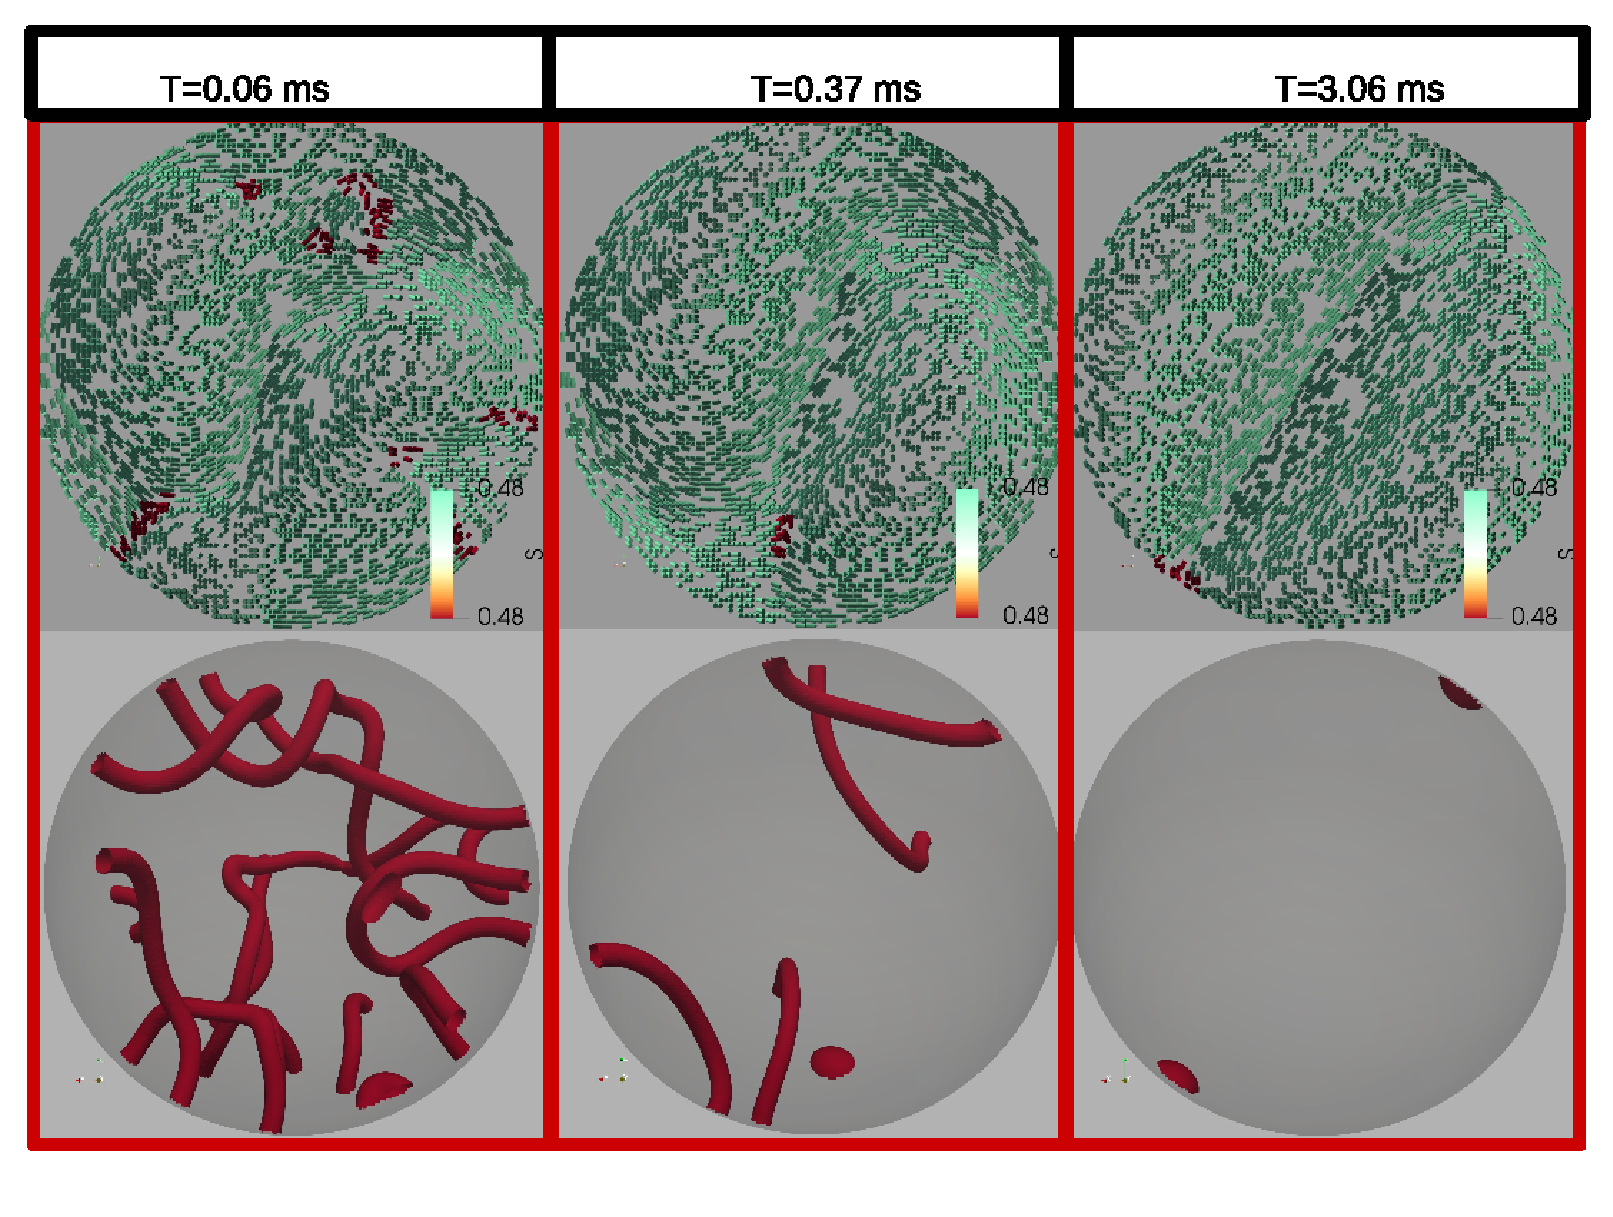
\includegraphics[width=\linewidth]{n=2.eps}
	%\vspace{-1.0cm}
	\caption{twisted bipolar structure (TBS)}
	\label{n=2}
\end{figure*}

 LC droplets are often made by meticulously controlling the flow of two or more unmissable fluids, such as water and the LC material, in a microfluidic process []. In general, CLCs in spherical geometries present a myriad of possible metastable states depending on several parameters such as chirality, anchoring strength, anchoring kind and elastic constants. Here, we explore two different examples, both starting from a randomly oriented sample and executing a so-called thermal quenching, in which the droplet is quickly cooled from the isotropic state to the LC state. In the first case, shown in figure~\ref{n=2}, the directors (top) and the isosurfaces (bottom) are shown for three different times, viewed from the $xz$ axis. Here, we assume a radius-to-pitch ratio ($N=4R/p$, where $R$ is the radius of the droplet and $p$ is the CLC pitch) $N=2$ and that the droplets are subjected to strong planar anchoring.  The left column shows the directors organization (top) and the defect lines for $t=0.06$ ms. In the top figures, the red colored directors represent the position where defect lines cross that plane. For such short times, the organization is very random and the number of defect lines high. The middle column shows the droplet for $t=0.37$ ms, where the number of defect lines has decreased (annealing of defects) and the director organization (top) becomes more organized and the right-side column shows the final organization at $t=3.06$ ms. The final structure is known as twisted bipolar structure (TBS), with two boojums (surface defect) at the antipodal position, shown in the bottom figure. Notice that the defect annealing process here represented is the solution for the Beris-Edwards  equation, so one can use Marlics to study defect dynamics for several different parameters in spherical geometries. Also, one can study non-chiral situation (nematic) by making the pitch ($p$) infinity, so $N=0$.



\section{Conclusions}

In conclusion, we have presented marlics. Marlics is open source and
offers some of the most common cases for device simulation. Moreover
it provides a class organized framework where the user can program its
on cases if necessary.  

\label{sec:conclusions}

%% The Appendices part is started with the command \appendix;
%% appendix sections are then done as normal sections
 \appendix

\section{Software implementation and extension:}\label{apx:extending_marlics}

Marlics is subdivided in a series of C++ classes. There are 4 main
super classes which confers most of marlics usability : energy,
boundary, geometry and integrator. Each specific functionality must be
implemented deriving one of these classes, \textcolor{red}{for
  instance, the Landau-de Gennes energy is implemented through a class
  derived from the energy super class}. Maybe I should remove the
example. Follow in details what every of these class does and how to specialize it:

\begin{itemize}

\item Driver: We start with the driver helper class. Its main purpose
  it is to parses the input file and assembly the simulation pieces,
  except for the boundaries. Any new parameter that the user wants to
  include in the system must be added in the structure xxxx and later
  provided a reading keyword in the routine parse_input_file.


  
\item Energy: Energy super class contain the API to calculate the
  R.H.S. of equations \eqref{eq:dissipacao_Q_superficie}. Different
  from the other classes we provide an single bulk energy name given
  by \eqref{eq:total_energy}. In this way we can inline the routines
  in the code and allow a series of optimizations to be performed. We
  believe this is not a drawback since the user will be using the same
  bulk energy most of time. If the user wants to include a term in the
  bulk energy, we advise him/her to include the new term in the
  Landau-de Gennes class and keep the program structure.
  
\item Boundary is a specialization of energy, but still a super-class,
  which contains the API to call functions to calculate R.H.S of
  functions \eqref{eq:dissipacao_Q_superficie} and some variables
  containing information such as: Energy name and which boundary
  number. Any new boundary condition must be derived from this super
  class. After performing a derivation the user has to add an entry in
  the geometry class routine: setup_boundary_conditions. Containing
  the keyword that will be used in the input file.

\item Integrator contains the routine to evolve the system of
  equations. This super-class is very simple, it contains the routine
  \textit{evolve}, which will perform the time integration of the
  system of equations. However, much of the actual calculation is
  performed in the class geometry. Here the user must provide the
  coefficients of the integrator pieces and also a function to
  estimate the integration error.

\item Geometry contain the information about the geometry of the
  system and their boundary conditions. Here the user must provide a
  way to calculate the boundaries normals, and the parameter field
  derivatives. With all inofrmation present in the geometry class, we
  put the calculation of RHS in it, therefore, there is a routine to
  calculate the evolution RHS. To do this the geoemtry has as member
  an energy instance and a linked list containing the boundaries
  pointers.


\end{itemize}

 
\section{List of available parameters and its units:}
 \label{apx:list_of_parameters}

 \onecolumn
 \begin{center}
	\begin{longtable}{|c|c|c|c|}
          \hline 
          Parameter name  & variable type	& units & mandatory/standard value\\ 
          \hline 
          {Geometry}	& string & 	& Yes  \\ 
          \hline 
          {Nx}	& integer &	& Yes \\ 
          \hline                                  
          {Ny}	& integer &      & Yes \\ 
          \hline                                  
          {Nz}	& integer &      & Yes \\ 
          \hline                                  
          {dx}	& real & nm      & Yes \\ 
          \hline                                  
          {dy}	& real & nm   & Yes \\ 
          \hline                                  
          {dz}	& real & nm	& Yes \\ 
          \hline 
          {integrator}	& string & & Yes\\ 
          \hline 
          facmin	& real &   & 0.4\\ 
          \hline 
          facmax	& real &   & 3\\ 
          \hline 
          prefac	& real &  & 0.8\\ 
          \hline 
          Atol	& real &  &0.001\\ 
          \hline 
          Rtol & real &  &0.001\\ 
          \hline 
          {a} & real& MJ$/(m^2 K)$ & Yes\\
          \hline 
          {b} & real& MJ$/m^2$ & Yes\\ 
          \hline
          {c} & real& MJ$/m^2$ & Yes\\ 
          \hline 
          {K1} & real &  pN  &  See \ref{sec:software_usage}\\ 
          \hline
          {K2} & real &  pN  &  See \ref{sec:software_usage}\\ 
          \hline
          {K3} & real &  pN  &  See \ref{sec:software_usage}\\ 
          \hline 
          {L1} & real &  pN & See \ref{sec:software_usage}\\ 
          \hline 
          {L2} & real &  pN & No   \\ 
          \hline
          { L3} & real & pN & No   \\ 
          \hline
          { Ls} & real & pN & No   \\ 
          \hline
          { Lq} & real & pN/m & No   \\ 
          \hline 
          {p0 or q0} & real & nm or 1/nm & No \\ 
          \hline
          {T}  & real & K	& No \\ 
          \hline 
          {Mu or gamma} & real & Pa/s & Yes \\ 
          \hline 
          {Mu\_s or gamma\_s} & real & nm Pa m/s&  See \ref{sec:software_usage}\\ 
          \hline 
          {ti}& real & $\mu$s  & 0.0 \\ 
          \hline 
          {tf}& real & $\mu$s  & Yes\\ 
          \hline 
          {dt}& real & $\mu$s  & Tf/1e6 \\ 
          \hline 
          {timeprint}& real & $\mu$s &  Tf/20 \\ 
          \hline 
          {timeprint\_type}& string &  & Linear\\ 
          \hline 
          {timeprint\_increase\_factor}& real&   & Tf/20 \\ 
          \hline 
          {output\_folder}&	string & & . \\ 
          \hline 
          {output\_fname}&	string & & director\_field\_\$\$.csv \\ 
          \hline 
          {initial\_output\_file\_number} & int & & 0 \\ 
          \hline 
          {initial\_conditions} & string & & yes \\ 
          \hline 
          {initial\_file\_name} & string & & See \ref{sec:software_usage} \\ 
          \hline 
          {theta\_i} &	real & degrees & See \ref{sec:software_usage} \\ 
          \hline 
          {phi\_i} &	real & degrees  & See \ref{sec:software_usage}\\ 
          \hline 
          {anchoring\_type} & int + string & & See \ref{sec:software_usage}\\ 
          \hline 
          {Wo1}& int + real & &  See \ref{sec:software_usage}  \\ 
          \hline 
          {theta\_0} &  int + real  & & See \ref{sec:software_usage} \\ 
          \hline 
          {phi\_0} &	 int + real  & & See \ref{sec:software_usage} \\ 
          \hline 
	\end{longtable} 
\end{center}
\twocolumn
 
 \section{Input File example:}
 \label{apx:input_file}

 Here you can find the complete input file:
\onecolumn
\begin{lstlisting}	

   #Geometry Parameters:
   geometry  slab
   Nx  200                /*      grid size      */
   Ny  200                /*      grid size      */
   Nz  100                /*      grid size      */
   dx  10.0               /*      10^-9 m         */
   dy  10.0               /*      10^-9 m         */
   dz  10.0               /*      10^-9 m         */


  #Integrator parameters:
  integrator  DP5
  atol 0.005
  rtol 0.005
  facmax 3.0
  facmin 0.4
  prefac 0.8


  #Liquid crystal parameters:
  a   0.182
  b  -2.12
  c  1.73
  T -1            Kelvin
  k11  16.7        /*   pN   */
  k22  7.8         /*   pN   */
  k33  18.1        /*   pN   */
  k24  0           /*   pN   */ 
  p0  500
  mu_1     0.3          /*     Pa s            */
  mu_1_s   30.0          /*    Pa nm s     */


  #Time parameters:
  dt  0.001            /*     10^-6 s         */	
  ti  0.0              /*     10^-6 s         */	
  tf  5000.0           /*     10^-6 s         */

  #Output Parameters:
   time_print_type             logarithmic
   timeprint                   50.        /*  10^-6 s   */
   timeprint_increase_factor   1.16            
   output_folder               .
   output_fname                output_$$.csv
   initial_output_file_number  0	

   #Initial conditions:
   initial_conditions  random


   #Boundaries conditions

   #Bottom boundaries:
   anchoring_type 0  Rapini-Papoular
   Wo1            0  1000.0
   theta_0        0  45.0
   phi_0          0  45.0	

   #Top boundaries:
   anchoring_type 1  Fournier-Galatola
   Wo1            1  1000.0

\end{lstlisting}
\twocolumn

\section{Output file:}\label{apx:output_file}
 
%% References
%%
%% Following citation commands can be used in the body text:
%% Usage of \cite is as follows:
%%   \cite{key}         ==>>  [#]
%%   \cite[chap. 2]{key} ==>> [#, chap. 2]
%%

%% References with bibTeX database:

\bibliographystyle{elsarticle-num}
\bibliography{marlics}

%% Authors are advised to submit their bibtex database files. They are
%% requested to list a bibtex style file in the manuscript if they do
%% not want to use elsarticle-num.bst.

%% References without bibTeX database:

% \begin{thebibliography}{00}

%% \bibitem must have the following form:
%%   \bibitem{key}...
%%

% \bibitem{}

% \end{thebibliography}


\end{document}

%%
%% End of file \documentclass[a4paper,onecolumn,12pt]{article}

